% Options for packages loaded elsewhere
\PassOptionsToPackage{unicode}{hyperref}
\PassOptionsToPackage{hyphens}{url}
%
\documentclass[
  12pt,
]{book}
\usepackage{amsmath,amssymb}
\usepackage{lmodern}
\usepackage{ifxetex,ifluatex}
\ifnum 0\ifxetex 1\fi\ifluatex 1\fi=0 % if pdftex
  \usepackage[T1]{fontenc}
  \usepackage[utf8]{inputenc}
  \usepackage{textcomp} % provide euro and other symbols
\else % if luatex or xetex
  \usepackage{unicode-math}
  \defaultfontfeatures{Scale=MatchLowercase}
  \defaultfontfeatures[\rmfamily]{Ligatures=TeX,Scale=1}
\fi
% Use upquote if available, for straight quotes in verbatim environments
\IfFileExists{upquote.sty}{\usepackage{upquote}}{}
\IfFileExists{microtype.sty}{% use microtype if available
  \usepackage[]{microtype}
  \UseMicrotypeSet[protrusion]{basicmath} % disable protrusion for tt fonts
}{}
\makeatletter
\@ifundefined{KOMAClassName}{% if non-KOMA class
  \IfFileExists{parskip.sty}{%
    \usepackage{parskip}
  }{% else
    \setlength{\parindent}{0pt}
    \setlength{\parskip}{6pt plus 2pt minus 1pt}}
}{% if KOMA class
  \KOMAoptions{parskip=half}}
\makeatother
\usepackage{xcolor}
\IfFileExists{xurl.sty}{\usepackage{xurl}}{} % add URL line breaks if available
\IfFileExists{bookmark.sty}{\usepackage{bookmark}}{\usepackage{hyperref}}
\hypersetup{
  pdftitle={BIO8940 Advanced stats and Open Science},
  pdfauthor={Julien Martin},
  hidelinks,
  pdfcreator={LaTeX via pandoc}}
\urlstyle{same} % disable monospaced font for URLs
\usepackage{color}
\usepackage{fancyvrb}
\newcommand{\VerbBar}{|}
\newcommand{\VERB}{\Verb[commandchars=\\\{\}]}
\DefineVerbatimEnvironment{Highlighting}{Verbatim}{commandchars=\\\{\}}
% Add ',fontsize=\small' for more characters per line
\usepackage{framed}
\definecolor{shadecolor}{RGB}{248,248,248}
\newenvironment{Shaded}{\begin{snugshade}}{\end{snugshade}}
\newcommand{\AlertTok}[1]{\textcolor[rgb]{0.94,0.16,0.16}{#1}}
\newcommand{\AnnotationTok}[1]{\textcolor[rgb]{0.56,0.35,0.01}{\textbf{\textit{#1}}}}
\newcommand{\AttributeTok}[1]{\textcolor[rgb]{0.77,0.63,0.00}{#1}}
\newcommand{\BaseNTok}[1]{\textcolor[rgb]{0.00,0.00,0.81}{#1}}
\newcommand{\BuiltInTok}[1]{#1}
\newcommand{\CharTok}[1]{\textcolor[rgb]{0.31,0.60,0.02}{#1}}
\newcommand{\CommentTok}[1]{\textcolor[rgb]{0.56,0.35,0.01}{\textit{#1}}}
\newcommand{\CommentVarTok}[1]{\textcolor[rgb]{0.56,0.35,0.01}{\textbf{\textit{#1}}}}
\newcommand{\ConstantTok}[1]{\textcolor[rgb]{0.00,0.00,0.00}{#1}}
\newcommand{\ControlFlowTok}[1]{\textcolor[rgb]{0.13,0.29,0.53}{\textbf{#1}}}
\newcommand{\DataTypeTok}[1]{\textcolor[rgb]{0.13,0.29,0.53}{#1}}
\newcommand{\DecValTok}[1]{\textcolor[rgb]{0.00,0.00,0.81}{#1}}
\newcommand{\DocumentationTok}[1]{\textcolor[rgb]{0.56,0.35,0.01}{\textbf{\textit{#1}}}}
\newcommand{\ErrorTok}[1]{\textcolor[rgb]{0.64,0.00,0.00}{\textbf{#1}}}
\newcommand{\ExtensionTok}[1]{#1}
\newcommand{\FloatTok}[1]{\textcolor[rgb]{0.00,0.00,0.81}{#1}}
\newcommand{\FunctionTok}[1]{\textcolor[rgb]{0.00,0.00,0.00}{#1}}
\newcommand{\ImportTok}[1]{#1}
\newcommand{\InformationTok}[1]{\textcolor[rgb]{0.56,0.35,0.01}{\textbf{\textit{#1}}}}
\newcommand{\KeywordTok}[1]{\textcolor[rgb]{0.13,0.29,0.53}{\textbf{#1}}}
\newcommand{\NormalTok}[1]{#1}
\newcommand{\OperatorTok}[1]{\textcolor[rgb]{0.81,0.36,0.00}{\textbf{#1}}}
\newcommand{\OtherTok}[1]{\textcolor[rgb]{0.56,0.35,0.01}{#1}}
\newcommand{\PreprocessorTok}[1]{\textcolor[rgb]{0.56,0.35,0.01}{\textit{#1}}}
\newcommand{\RegionMarkerTok}[1]{#1}
\newcommand{\SpecialCharTok}[1]{\textcolor[rgb]{0.00,0.00,0.00}{#1}}
\newcommand{\SpecialStringTok}[1]{\textcolor[rgb]{0.31,0.60,0.02}{#1}}
\newcommand{\StringTok}[1]{\textcolor[rgb]{0.31,0.60,0.02}{#1}}
\newcommand{\VariableTok}[1]{\textcolor[rgb]{0.00,0.00,0.00}{#1}}
\newcommand{\VerbatimStringTok}[1]{\textcolor[rgb]{0.31,0.60,0.02}{#1}}
\newcommand{\WarningTok}[1]{\textcolor[rgb]{0.56,0.35,0.01}{\textbf{\textit{#1}}}}
\usepackage{longtable,booktabs,array}
\usepackage{calc} % for calculating minipage widths
% Correct order of tables after \paragraph or \subparagraph
\usepackage{etoolbox}
\makeatletter
\patchcmd\longtable{\par}{\if@noskipsec\mbox{}\fi\par}{}{}
\makeatother
% Allow footnotes in longtable head/foot
\IfFileExists{footnotehyper.sty}{\usepackage{footnotehyper}}{\usepackage{footnote}}
\makesavenoteenv{longtable}
\usepackage{graphicx}
\makeatletter
\def\maxwidth{\ifdim\Gin@nat@width>\linewidth\linewidth\else\Gin@nat@width\fi}
\def\maxheight{\ifdim\Gin@nat@height>\textheight\textheight\else\Gin@nat@height\fi}
\makeatother
% Scale images if necessary, so that they will not overflow the page
% margins by default, and it is still possible to overwrite the defaults
% using explicit options in \includegraphics[width, height, ...]{}
\setkeys{Gin}{width=\maxwidth,height=\maxheight,keepaspectratio}
% Set default figure placement to htbp
\makeatletter
\def\fps@figure{htbp}
\makeatother
\setlength{\emergencystretch}{3em} % prevent overfull lines
\providecommand{\tightlist}{%
  \setlength{\itemsep}{0pt}\setlength{\parskip}{0pt}}
\setcounter{secnumdepth}{5}
%\usepackage{booktabs}
\usepackage{ctable}
\usepackage{fancyhdr}
\usepackage{float}
\usepackage[margin=2cm]{geometry}

\floatplacement{figure}{H}

%\usepackage[sf,bf]{titlesec}

\hypersetup{colorlinks=true, urlcolor=blue}

\renewcommand{\chaptername}{Chapitre}
\renewcommand{\contentsname}{Table des Matières}
\renewcommand{\partname}{Partie}

\usepackage{framed,color}
\definecolor{incolor}{RGB}{240,240,240}
\definecolor{outcolor}{RGB}{248,248,248}

\renewcommand{\textfraction}{0.05}
\renewcommand{\topfraction}{0.8}
\renewcommand{\bottomfraction}{0.8}
\renewcommand{\floatpagefraction}{0.75}

%\renewenvironment{quote}{\begin{VF}}{\end{VF}}

\ifxetex
 \usepackage{letltxmacro}
 \setlength{\XeTeXLinkMargin}{1pt}
 \LetLtxMacro\SavedIncludeGraphics\includegraphics
 \def\includegraphics#1#{% #1 catches optional stuff (star/opt. arg.)
   \IncludeGraphicsAux{#1}%
 }%
 \newcommand*{\IncludeGraphicsAux}[2]{%
   \XeTeXLinkBox{%
     \SavedIncludeGraphics#1{#2}%
   }%
 }%
\fi

\makeatletter
\newenvironment{kframe}{%
\medskip{}
\setlength{\fboxsep}{.8em}
\def\at@end@of@kframe{}%
\ifinner\ifhmode%
 \def\at@end@of@kframe{\end{minipage}}%
 \begin{minipage}{\columnwidth}%
\fi\fi%
\def\FrameCommand##1{\hskip\@totalleftmargin \hskip-\fboxsep
\colorbox{incolor}{##1}\hskip-\fboxsep
    % There is no \\@totalrightmargin, so:
    \hskip-\linewidth \hskip-\@totalleftmargin \hskip\columnwidth}%
\MakeFramed {\advance\hsize-\width
  \@totalleftmargin\z@ \linewidth\hsize
  \@setminipage}}%
{\par\unskip\endMakeFramed%
\at@end@of@kframe}
\makeatother

\makeatletter
\@ifundefined{Shaded}{
}{\renewenvironment{Shaded}{\begin{kframe}}{\end{kframe}}}
\makeatother

% \let\oldverbatim\verbatim
% \renewenvironment{Shaded}{\vspace{0.2cm}\begin{kframe}}{\end{kframe}}
% \renewenvironment{verbatim}{\begin{shaded}\begin{oldverbatim}}{\end{oldverbatim}\end{shaded}}

\newenvironment{rmdblock}[1]
 {
 \begin{itemize}
 \renewcommand{\labelitemi}{
   \raisebox{-.7\height}[0pt][0pt]{
     {\setkeys{Gin}{width=3em,keepaspectratio}\includegraphics{images/icons/#1}}
   }
 }
 \begin{kframe}
 \setlength{\fboxsep}{1em}
 \item
 }
 {
 \end{kframe}
 \end{itemize}
 }
\newenvironment{rmdnote}
  {\begin{rmdblock}{note}}
  {\end{rmdblock}}
\newenvironment{rmdcaution}
  {\begin{rmdblock}{caution}}
  {\end{rmdblock}}
\newenvironment{rmdimportant}
  {\begin{rmdblock}{important}}
  {\end{rmdblock}}
\newenvironment{rmdtip}
  {\begin{rmdblock}{tip}}
  {\end{rmdblock}}
\newenvironment{rmdwarning}
  {\begin{rmdblock}{warning}}
  {\end{rmdblock}}
\newenvironment{rmdcode}
  {\begin{rmdblock}{code}}
  {\end{rmdblock}}

\usepackage{makeidx}
\makeindex

\urlstyle{tt}

\usepackage{amsthm}
\makeatletter
\def\thm@space@setup{%
  \thm@preskip=8pt plus 2pt minus 4pt
  \thm@postskip=\thm@preskip
}
\makeatother

% \frontmatter
\ifluatex
  \usepackage{selnolig}  % disable illegal ligatures
\fi
\usepackage[]{natbib}
\bibliographystyle{apalike}

\title{BIO8940 Advanced stats and Open Science}
\usepackage{etoolbox}
\makeatletter
\providecommand{\subtitle}[1]{% add subtitle to \maketitle
  \apptocmd{\@title}{\par {\large #1 \par}}{}{}
}
\makeatother
\subtitle{Work in Progress}
\author{Julien Martin}
\date{16-02-2021}

\begin{document}
\maketitle

%\cleardoublepage\newpage\thispagestyle{empty}\null
%\cleardoublepage\newpage\thispagestyle{empty}\null
%\cleardoublepage\newpage
%\thispagestyle{empty}
%\begin{center}
%
\includegraphics{images/missing.png}
%\end{center}

%\setlength{\abovedisplayskip}{-5pt}
%\setlength{\abovedisplayshortskip}{-5pt}

{
\setcounter{tocdepth}{1}
\tableofcontents
}
\hypertarget{note}{%
\chapter*{Note}\label{note}}
\addcontentsline{toc}{chapter}{Note}

\begin{rmdimportant}
Work in progress. New chapters are going to appears regularly meaning that if you download the pdf it might be incomplete by the time we do the practical in class.
\end{rmdimportant}

\hypertarget{pruxe9face}{%
\chapter*{Préface}\label{pruxe9face}}
\addcontentsline{toc}{chapter}{Préface}

Les exercices de laboratoire que vous retrouverez dans les pages qui suivent sont conçus de manière à vous permettre de développer une expérience pratique en analyse de données à l'aide d'un logiciel (R).
R est un logiciel très puissant, mais comme tous les logiciels, il a des limites.
En particulier il ne peut réfléchir à votre place, vous dire si l'analyse que vous tentez d'effectuer est appropriée ou sensée, ou interpréter biologiquement les résultats.

\hypertarget{quelques-points-importants-uxe0-retenir}{%
\section*{Quelques points importants à retenir}\label{quelques-points-importants-uxe0-retenir}}
\addcontentsline{toc}{section}{Quelques points importants à retenir}

\begin{itemize}
\item
  Avant de commencer une analyse statistique, il faut d'abord vous familiariser son fonctionnement.
  Cela ne veut pas dire que vous devez connaître les outils mathématiques qui la sous-tendent, mais vous devriez au moins comprendre les principes utilisés lors de cette analyse.
  Avant de faire un exercice de laboratoire, lisez donc la section correspondante dans les notes de cours.
  Sans cette lecture préalable, il est très probable que les résultats produits par le logiciel, même si l'analyse a été effectuée correctement, seront indéchiffrables.
\item
  Les laboratoires sont conçus pour compléter les cours théoriques et vice versa.
  À cause des contraintes d'horaires, il se pourrait que le cours et le laboratoire ne soient pas parfaitement synchronisés.
  N'hésitez donc pas à poser des questions sur le labo en classe ou des questions théoriques au laboratoire.
\item
  Travaillez sur les exercices de laboratoire à votre propre rythme.
  Certains exercices prennent beaucoup moins de temps que d'autres et il n'est pas nécessaire de compléter un exercice par séance de laboratoire.
  En fait deux séances de laboratoire sont prévues pour certains des exercices.
  Même si vous n'êtes pas notés sur les exercices de laboratoire, soyez conscient que ces exercices
  sont essentiels.
  Si vous ne les faites pas, il est très peu probable que vous serez capable de compléter les devoirs et le projet de session.
  Prenez donc ces exercices de laboratoire au sérieux !
\item
  Les 2 premier laboratoires sont conçu pour vous permettre d'acquérir ou de réviser le minimum de connaissances requises pour vous permettre de réaliser les exercices de laboratoires avec R.
  Il y a presque toujours de multiples façons de faire les choses avec R et vous ne trouverez ici que des méthodes simples.
  Ceux et celles d'entre vous qui y sont enclins pourront trouver en ligne des instructions plus détaillées et complexes.
  En particulier, je vous conseille :

  \begin{itemize}
  \tightlist
  \item
    R pour les débutants
    \url{http://cran.r-project.org/doc/contrib/Paradis-rdebuts_fr.pdf}
  \item
    An introduction to R
    \url{http://cran.r-project.org/doc/manuals/R-intro.html}
  \item
    Si vous préférez des manuels, le site web de CRAN en garde une liste commentée à :
    \url{http://www.r-project.org/doc/bib/R-books.html}
  \item
    Une liste impressionnante de très bon livre sur R
    \url{https://www.bigbookofr.com/}
  \item
    Finalement, comme aide-mémoire à garder sous la main, je vous recommande R reference card par Tom Short
    \url{http://cran.r-project.org/doc/contrib/Short-refcard.pdf}
  \end{itemize}
\end{itemize}

\hypertarget{quest-ce-que-r-et-pourquoi-lutiliser-dans-ce-cours}{%
\section*{Qu'est-ce que R et pourquoi l'utiliser dans ce cours?}\label{quest-ce-que-r-et-pourquoi-lutiliser-dans-ce-cours}}
\addcontentsline{toc}{section}{Qu'est-ce que R et pourquoi l'utiliser dans ce cours?}

R est un logiciel libre et multi-plateforme formant un système statistique et graphique.
R est également un langage de programmation spécialisé pour les statistiques.

R a deux très grands avantages pour ce cours, et un inconvénient embêtant initialement mais qui vous forcera à acquérir des excellentes habitudes de travail.
Le premier avantage est que vous pouvez tous l'installer sur votre (ou vos) ordinateurs personnel gratuitement.
C'est important parce que c'est à l'usage que vous apprendrez et maîtriserez réellement les biostatistiques et cela implique que vous devez avoir un accès facile et illimité à un logiciel statistique.
Le deuxième avantage est que R peut tout faire en statistiques.
R est conçu pour être extensible et est devenu l'outil de prédilection des statisticiens mondialement.
La question n'est plus : " Est-ce que R peut faire ceci? ``, mais devient'' Comment faire ceci avec R ".
Et la recherche internet est votre ami.
Aucun autre logiciel n'offre ces deux avantages.

L'inconvénient embêtant initialement est que l'on doit opérer R en tapant des instructions (ou en copiant des sections de code) plutôt qu'en utilisant des menus et en cliquant sur différentes options.
Si on ne sait pas quelle commande taper, rien ne se passe.
Ce n'est donc pas facile d'utilisation à priori.
Cependant, il est possible d'apprendre rapidement à faire certaines des opérations de base (ouvrir un fichier de données, faire un graphique pour examiner ces données, effectuer un test statistique simple).
Et une fois que l'on comprend le principe de la chose, on peut assez facilement trouver sur le web des exemples d'analyses ou de graphiques plus complexes et adapter le code à nos propres besoins.
C'est ce que vous ferez dans le premier laboratoire pour vous familiariser avec R.

Pourquoi cet inconvénient est-il d'une certaine façon un avantage? Parce que vous allez sauver du temps en fin de compte.
Garanti.
Croyez-moi, on ne fait jamais une analyse une seule fois.
En cours de route, on découvre des erreurs d'entrée de données, ou que l'on doit faire l'analyse séparément pour des sous-groupes, ou on obtient des données supplémentaires, ou on fait une erreur.
On doit alors recommencer l'analyse.
Avec une interface graphique et des menus, cela implique recommencer à cliquer ici, entre des paramètres dans des boîtes et sélectionner des boutons.
Chaque fois avec possibilité d'erreur.
Avec une série de commandes écrites, il suffit de corriger ce qui doit l'être puis de copier-coller l'ensemble pour répéter instantanément.
Et vous avez la possibilité de parfaitement documenter ce que vous avez fait.
C'est comme cela que les professionnels travaillent et offrent une assurance de qualité de leurs résultats.

\hypertarget{installation-des-logiciels-nuxe9cessaires}{%
\section*{Installation des logiciels nécessaires}\label{installation-des-logiciels-nuxe9cessaires}}
\addcontentsline{toc}{section}{Installation des logiciels nécessaires}

\hypertarget{r}{%
\subsection*{R}\label{r}}
\addcontentsline{toc}{subsection}{R}

Pour installer R sur un nouvel ordinateur, allez au site \url{http://cran.r-project.org/}.
Vous y trouverez des versions compilées (binaries) ou non (sources) pour votre système d'exploitation de prédilection (Windows, MacOS, Linux).

Note : R a déjà été installé sur les ordinateurs du laboratoire (la version pourrait être un peu plus ancienne, mais cela devrait être sans conséquences).

\hypertarget{text-editor-or-ide}{%
\subsection{Text editor or IDE}\label{text-editor-or-ide}}

Tinn-r
Atom sublime, emacs, vim

\hypertarget{rstudio}{%
\subsubsection*{Rstudio}\label{rstudio}}
\addcontentsline{toc}{subsubsection}{Rstudio}

RStudio est un environnement de développement intégré (IDE) créé spécifiquement pour travailler avec R. Sa popularité connaît une progression foudroyante depuis 2014.
Il permet de consulter dans une interface conviviale ses fichiers de script, la ligne de commande R, les rubriques d'aide,
les graphiques, etc.

RStudio est disponible à l'identique pour les plateformes Windows, OS X et Linux.
Pour une utilisation locale sur son poste de travail, on installera la version libre (Open Source) de RStudio Desktop depuis le site
\url{https://www.rstudio.com/products/rstudio/download/}

\hypertarget{visual-studio-code}{%
\subsubsection*{Visual Studio Code}\label{visual-studio-code}}
\addcontentsline{toc}{subsubsection}{Visual Studio Code}

\hypertarget{tinn-r}{%
\subsubsection*{Tinn-r}\label{tinn-r}}
\addcontentsline{toc}{subsubsection}{Tinn-r}

\hypertarget{paquets-pour-r}{%
\subsection*{Paquets pour R}\label{paquets-pour-r}}
\addcontentsline{toc}{subsection}{Paquets pour R}

\begin{itemize}
\tightlist
\item
  Rmarkdown
\item
  tinytex
\end{itemize}

Ces 2 paquets devrait être installé automatiquement avec RStudio, mais pas toujours. Je vous recommande donc de les installer manuellement. Pour ce faire, simplement copier-coller le texte suivant dans le terminal R.

\begin{Shaded}
\begin{Highlighting}[]
\FunctionTok{install.packages}\NormalTok{(}\FunctionTok{c}\NormalTok{(}\StringTok{"rmarkdown"}\NormalTok{, }\StringTok{"tinytex"}\NormalTok{))}
\end{Highlighting}
\end{Shaded}

\hypertarget{pandoc}{%
\subsection*{pandoc}\label{pandoc}}
\addcontentsline{toc}{subsection}{pandoc}

\hypertarget{latex}{%
\subsection*{laTex}\label{latex}}
\addcontentsline{toc}{subsection}{laTex}

\begin{itemize}
\tightlist
\item
  tinytex
  or others
\end{itemize}

\hypertarget{instructions-guxe9nuxe9rales-pour-les-laboratoires}{%
\section*{Instructions générales pour les laboratoires}\label{instructions-guxe9nuxe9rales-pour-les-laboratoires}}
\addcontentsline{toc}{section}{Instructions générales pour les laboratoires}

\begin{itemize}
\tightlist
\item
  Apporter une clé USB ou son équivalent à chaque séance de laboratoire pour sauvegarder votre travail.
\item
  Lire l'exercice de laboratoire AVANT la séance, lire le code R correspondant et préparer vos questions sur le code.
\item
  Durant les pré-labs, écouter les instructions et posez vos questions au moment approprié.
\item
  Faites les exercices du manuel de laboratoire à votre rythme, en équipe, puis je vous recommande de commencer (compléter?) le devoir.
  Profitez de la présence du démonstrateur et du prof\ldots{}
\item
  Pendant vos analyses, copiez-collez des fragments de sorties de R dans un document (par exemple dans votre traitement de texte favori) et annotez abondamment.
\item
  Ne tapez pas directement vos commandes dans R mais plutôt dans un script.
  Vous pourrez ainsi refaire le labo instantanément, récupérer des fragments de code, ou plus facilement identifier les erreurs dans vos analyses.
\item
  Créez votre propre librairie de fragments de codes (snippets).
  Annotez-là abondamment.
  Vous vous en féliciterez plus tard.
\end{itemize}

\hypertarget{notes-sur-le-manuel}{%
\section*{Notes sur le manuel}\label{notes-sur-le-manuel}}
\addcontentsline{toc}{section}{Notes sur le manuel}

Vous trouverez dans le manuel des explications sur la théorie, du code R, des explications sur R et des exercises.

Le manuel essaie aussi de mettre en évidence le texte de différentes manières.

\begin{rmdcode}
Avec des sections à vous de jouer, ui indique un exercise à faire, idéalement sans regarder la solution qui se trouve plus bas.
\end{rmdcode}

\begin{rmdcaution}
des avertissements
\end{rmdcaution}

\begin{rmdwarning}
des avertissements
\end{rmdwarning}

\begin{rmdimportant}
des points importants
\end{rmdimportant}

\begin{rmdnote}
des notes
\end{rmdnote}

\begin{rmdtip}
et des conseils
\end{rmdtip}
\#\#\# Resources \{-\}

Ce document est généré par l'excellente extension \href{https://bookdown.org/}{bookdown} de \href{https://yihui.name/}{Yihui Xie}. Il est basé sur le précédent manuel de laboratoire \emph{BIO4558 manuel de laboratoire} par Antoine Morin. L'introduction à R est largement reprise de l'excellent manuel de \textbf{Julien Barnier} intitulé \href{https://juba.github.io/tidyverse/}{\emph{Introduction à R et au tidyverse}}

\hypertarget{licence}{%
\subsection*{Licence}\label{licence}}
\addcontentsline{toc}{subsection}{Licence}

Ce document est mis à disposition selon les termes de la \href{http://creativecommons.org/licenses/by-nc-sa/4.0/}{Licence Creative Commons Attribution - Pas d'Utilisation Commerciale - Partage dans les Mêmes Conditions 4.0 International}.

\begin{figure}
\centering

\includegraphics{images/icons/license_cc.png}
\caption{Licence Creative Commons}
\end{figure}

\hypertarget{part-open-science}{%
\part{Open Science}\label{part-open-science}}

\hypertarget{introduction-to-open-science}{%
\chapter{Introduction to open Science}\label{introduction-to-open-science}}

\hypertarget{introduction-to-rmarkdown}{%
\chapter{Introduction to Rmarkdown}\label{introduction-to-rmarkdown}}

\hypertarget{introduction-to-github-with-r}{%
\chapter{Introduction to github with R}\label{introduction-to-github-with-r}}

\hypertarget{part-statistics}{%
\part{Statistics}\label{part-statistics}}

\hypertarget{refresher-on-glm}{%
\chapter{\texorpdfstring{Refresher on \texttt{glm}}{Refresher on glm}}\label{refresher-on-glm}}

\begin{Shaded}
\begin{Highlighting}[]
\NormalTok{m1 }\OtherTok{\textless{}{-}} \FunctionTok{glm}\NormalTok{(fish }\SpecialCharTok{\textasciitilde{}}\NormalTok{ french\_captain, }\AttributeTok{data =}\NormalTok{ dads\_joke, }\AttributeTok{family =}\NormalTok{ poisson)}
\end{Highlighting}
\end{Shaded}

\textbf{Exercice 5}

On a relevé les notes en maths, anglais et sport d'une classe de 6 élèves et on a stocké ces données dans trois vecteurs :

\begin{Shaded}
\begin{Highlighting}[]
\NormalTok{maths }\OtherTok{\textless{}{-}} \FunctionTok{c}\NormalTok{(}\DecValTok{12}\NormalTok{, }\DecValTok{16}\NormalTok{, }\DecValTok{8}\NormalTok{, }\DecValTok{18}\NormalTok{, }\DecValTok{6}\NormalTok{, }\DecValTok{10}\NormalTok{)}
\NormalTok{anglais }\OtherTok{\textless{}{-}} \FunctionTok{c}\NormalTok{(}\DecValTok{14}\NormalTok{, }\DecValTok{9}\NormalTok{, }\DecValTok{13}\NormalTok{, }\DecValTok{15}\NormalTok{, }\DecValTok{17}\NormalTok{, }\DecValTok{11}\NormalTok{)}
\NormalTok{sport }\OtherTok{\textless{}{-}} \FunctionTok{c}\NormalTok{(}\DecValTok{18}\NormalTok{, }\DecValTok{11}\NormalTok{, }\DecValTok{14}\NormalTok{, }\DecValTok{10}\NormalTok{, }\DecValTok{8}\NormalTok{, }\DecValTok{12}\NormalTok{)}
\end{Highlighting}
\end{Shaded}

Calculer la moyenne des élèves de la classe en anglais.

Calculer la moyenne générale de chaque élève.

\begin{verbatim}
## [1] 13.16667
\end{verbatim}

\begin{verbatim}
## [1] 14.66667 12.00000 11.66667 14.33333 10.33333 11.00000
\end{verbatim}

\textbf{Exercice 5}

On a relevé les notes en maths, anglais et sport d'une classe de 6 élèves et on a stocké ces données dans trois vecteurs :

\begin{Shaded}
\begin{Highlighting}[]
\NormalTok{maths }\OtherTok{\textless{}{-}} \FunctionTok{c}\NormalTok{(}\DecValTok{12}\NormalTok{, }\DecValTok{16}\NormalTok{, }\DecValTok{8}\NormalTok{, }\DecValTok{18}\NormalTok{, }\DecValTok{6}\NormalTok{, }\DecValTok{10}\NormalTok{)}
\NormalTok{anglais }\OtherTok{\textless{}{-}} \FunctionTok{c}\NormalTok{(}\DecValTok{14}\NormalTok{, }\DecValTok{9}\NormalTok{, }\DecValTok{13}\NormalTok{, }\DecValTok{15}\NormalTok{, }\DecValTok{17}\NormalTok{, }\DecValTok{11}\NormalTok{)}
\NormalTok{sport }\OtherTok{\textless{}{-}} \FunctionTok{c}\NormalTok{(}\DecValTok{18}\NormalTok{, }\DecValTok{11}\NormalTok{, }\DecValTok{14}\NormalTok{, }\DecValTok{10}\NormalTok{, }\DecValTok{8}\NormalTok{, }\DecValTok{12}\NormalTok{)}
\end{Highlighting}
\end{Shaded}

Calculer la moyenne des élèves de la classe en anglais.

Calculer la moyenne générale de chaque élève.

Test pour montrer la solution

\begin{verbatim}
## [1] 13.16667
\end{verbatim}

\begin{verbatim}
## [1] 14.66667 12.00000 11.66667 14.33333 10.33333 11.00000
\end{verbatim}

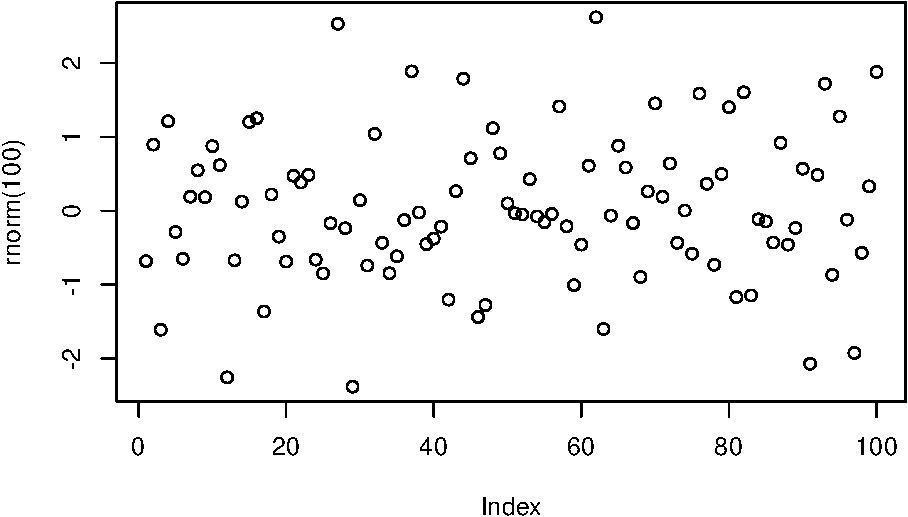
\includegraphics{BIO8940_book_files/figure-latex/unnamed-chunk-13-1.pdf}

\hypertarget{refresher-on-glm-1}{%
\chapter{\texorpdfstring{Refresher on \texttt{glm}}{Refresher on glm}}\label{refresher-on-glm-1}}

\begin{Shaded}
\begin{Highlighting}[]
\NormalTok{m1 }\OtherTok{\textless{}{-}} \FunctionTok{glm}\NormalTok{(fish }\SpecialCharTok{\textasciitilde{}}\NormalTok{ french\_captain, }\AttributeTok{data=}\NormalTok{ dads\_joke, }\AttributeTok{family =}\NormalTok{ poisson)}
\end{Highlighting}
\end{Shaded}

\textbf{Exercice 5}

On a relevé les notes en maths, anglais et sport d'une classe de 6 élèves et on a stocké ces données dans trois vecteurs :

\begin{Shaded}
\begin{Highlighting}[]
\NormalTok{maths }\OtherTok{\textless{}{-}} \FunctionTok{c}\NormalTok{(}\DecValTok{12}\NormalTok{, }\DecValTok{16}\NormalTok{, }\DecValTok{8}\NormalTok{, }\DecValTok{18}\NormalTok{, }\DecValTok{6}\NormalTok{, }\DecValTok{10}\NormalTok{)}
\NormalTok{anglais }\OtherTok{\textless{}{-}} \FunctionTok{c}\NormalTok{(}\DecValTok{14}\NormalTok{, }\DecValTok{9}\NormalTok{, }\DecValTok{13}\NormalTok{, }\DecValTok{15}\NormalTok{, }\DecValTok{17}\NormalTok{, }\DecValTok{11}\NormalTok{)}
\NormalTok{sport }\OtherTok{\textless{}{-}} \FunctionTok{c}\NormalTok{(}\DecValTok{18}\NormalTok{, }\DecValTok{11}\NormalTok{, }\DecValTok{14}\NormalTok{, }\DecValTok{10}\NormalTok{, }\DecValTok{8}\NormalTok{, }\DecValTok{12}\NormalTok{)}
\end{Highlighting}
\end{Shaded}

Calculer la moyenne des élèves de la classe en anglais.

Calculer la moyenne générale de chaque élève.

\begin{verbatim}
## [1] 13.16667
\end{verbatim}

\begin{verbatim}
## [1] 14.66667 12.00000 11.66667 14.33333 10.33333 11.00000
\end{verbatim}

\textbf{Exercice 5}

On a relevé les notes en maths, anglais et sport d'une classe de 6 élèves et on a stocké ces données dans trois vecteurs :

\begin{Shaded}
\begin{Highlighting}[]
\NormalTok{maths }\OtherTok{\textless{}{-}} \FunctionTok{c}\NormalTok{(}\DecValTok{12}\NormalTok{, }\DecValTok{16}\NormalTok{, }\DecValTok{8}\NormalTok{, }\DecValTok{18}\NormalTok{, }\DecValTok{6}\NormalTok{, }\DecValTok{10}\NormalTok{)}
\NormalTok{anglais }\OtherTok{\textless{}{-}} \FunctionTok{c}\NormalTok{(}\DecValTok{14}\NormalTok{, }\DecValTok{9}\NormalTok{, }\DecValTok{13}\NormalTok{, }\DecValTok{15}\NormalTok{, }\DecValTok{17}\NormalTok{, }\DecValTok{11}\NormalTok{)}
\NormalTok{sport }\OtherTok{\textless{}{-}} \FunctionTok{c}\NormalTok{(}\DecValTok{18}\NormalTok{, }\DecValTok{11}\NormalTok{, }\DecValTok{14}\NormalTok{, }\DecValTok{10}\NormalTok{, }\DecValTok{8}\NormalTok{, }\DecValTok{12}\NormalTok{)}
\end{Highlighting}
\end{Shaded}

Calculer la moyenne des élèves de la classe en anglais.

Calculer la moyenne générale de chaque élève.

Test pour montrer la solution

\begin{verbatim}
## [1] 13.16667
\end{verbatim}

\begin{verbatim}
## [1] 14.66667 12.00000 11.66667 14.33333 10.33333 11.00000
\end{verbatim}

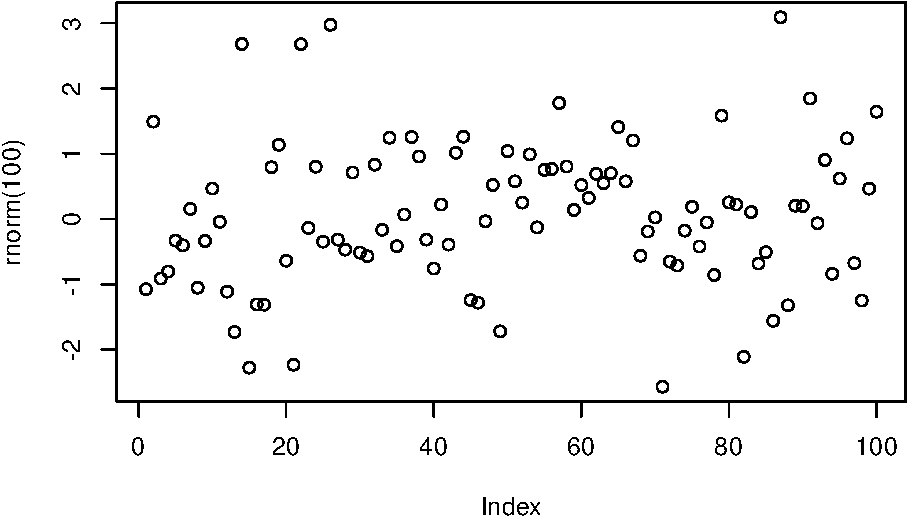
\includegraphics{BIO8940_book_files/figure-latex/unnamed-chunk-18-1.pdf}

\hypertarget{refresher-on-glm-2}{%
\chapter{\texorpdfstring{Refresher on \texttt{glm}}{Refresher on glm}}\label{refresher-on-glm-2}}

\begin{Shaded}
\begin{Highlighting}[]
\NormalTok{m1 }\OtherTok{\textless{}{-}} \FunctionTok{glm}\NormalTok{(fish }\SpecialCharTok{\textasciitilde{}}\NormalTok{ french\_captain, }\AttributeTok{data=}\NormalTok{ dads\_joke, }\AttributeTok{family =}\NormalTok{ poisson)}
\end{Highlighting}
\end{Shaded}

\textbf{Exercice 5}

On a relevé les notes en maths, anglais et sport d'une classe de 6 élèves et on a stocké ces données dans trois vecteurs :

\begin{Shaded}
\begin{Highlighting}[]
\NormalTok{maths }\OtherTok{\textless{}{-}} \FunctionTok{c}\NormalTok{(}\DecValTok{12}\NormalTok{, }\DecValTok{16}\NormalTok{, }\DecValTok{8}\NormalTok{, }\DecValTok{18}\NormalTok{, }\DecValTok{6}\NormalTok{, }\DecValTok{10}\NormalTok{)}
\NormalTok{anglais }\OtherTok{\textless{}{-}} \FunctionTok{c}\NormalTok{(}\DecValTok{14}\NormalTok{, }\DecValTok{9}\NormalTok{, }\DecValTok{13}\NormalTok{, }\DecValTok{15}\NormalTok{, }\DecValTok{17}\NormalTok{, }\DecValTok{11}\NormalTok{)}
\NormalTok{sport }\OtherTok{\textless{}{-}} \FunctionTok{c}\NormalTok{(}\DecValTok{18}\NormalTok{, }\DecValTok{11}\NormalTok{, }\DecValTok{14}\NormalTok{, }\DecValTok{10}\NormalTok{, }\DecValTok{8}\NormalTok{, }\DecValTok{12}\NormalTok{)}
\end{Highlighting}
\end{Shaded}

Calculer la moyenne des élèves de la classe en anglais.

Calculer la moyenne générale de chaque élève.

\begin{verbatim}
## [1] 13.16667
\end{verbatim}

\begin{verbatim}
## [1] 14.66667 12.00000 11.66667 14.33333 10.33333 11.00000
\end{verbatim}

\textbf{Exercice 5}

On a relevé les notes en maths, anglais et sport d'une classe de 6 élèves et on a stocké ces données dans trois vecteurs :

\begin{Shaded}
\begin{Highlighting}[]
\NormalTok{maths }\OtherTok{\textless{}{-}} \FunctionTok{c}\NormalTok{(}\DecValTok{12}\NormalTok{, }\DecValTok{16}\NormalTok{, }\DecValTok{8}\NormalTok{, }\DecValTok{18}\NormalTok{, }\DecValTok{6}\NormalTok{, }\DecValTok{10}\NormalTok{)}
\NormalTok{anglais }\OtherTok{\textless{}{-}} \FunctionTok{c}\NormalTok{(}\DecValTok{14}\NormalTok{, }\DecValTok{9}\NormalTok{, }\DecValTok{13}\NormalTok{, }\DecValTok{15}\NormalTok{, }\DecValTok{17}\NormalTok{, }\DecValTok{11}\NormalTok{)}
\NormalTok{sport }\OtherTok{\textless{}{-}} \FunctionTok{c}\NormalTok{(}\DecValTok{18}\NormalTok{, }\DecValTok{11}\NormalTok{, }\DecValTok{14}\NormalTok{, }\DecValTok{10}\NormalTok{, }\DecValTok{8}\NormalTok{, }\DecValTok{12}\NormalTok{)}
\end{Highlighting}
\end{Shaded}

Calculer la moyenne des élèves de la classe en anglais.

Calculer la moyenne générale de chaque élève.

Test pour montrer la solution

\begin{verbatim}
## [1] 13.16667
\end{verbatim}

\begin{verbatim}
## [1] 14.66667 12.00000 11.66667 14.33333 10.33333 11.00000
\end{verbatim}

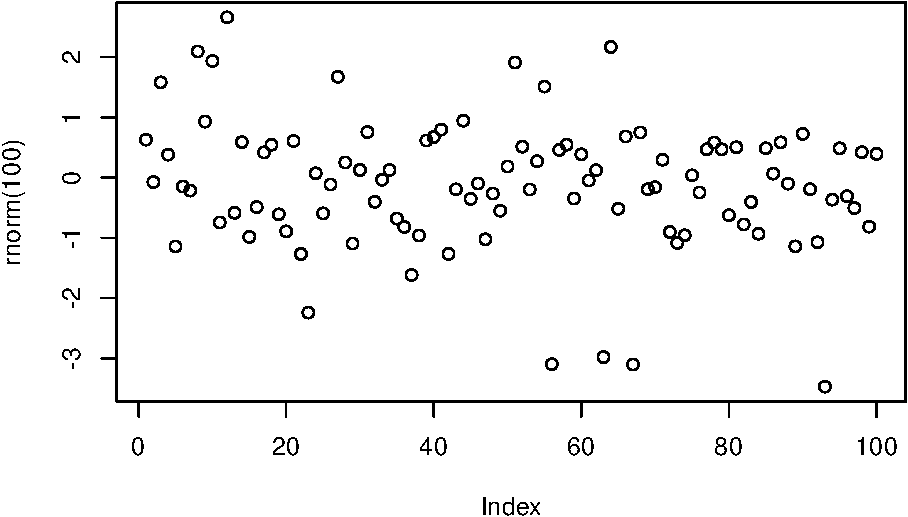
\includegraphics{BIO8940_book_files/figure-latex/unnamed-chunk-23-1.pdf}

\hypertarget{part-appendix}{%
\part{Appendix}\label{part-appendix}}

\hypertarget{r-1}{%
\chapter*{R}\label{r-1}}
\addcontentsline{toc}{chapter}{R}

  \bibliography{book.bib,packages.bib}

\printindex

\end{document}
